\chapter{Koja \v{z}ivotinja nam je donela SARS?}
\setbookcodestyle

\section{Uvod}
\label{sec:uvod}

Neka od glavnih pitanja koja mo\v{z}emo postaviti su:
Koja \v{z}ivotinja nam je donela SARS? Kako smo se prvobitno zarazili? Kako se SARS \v{s}irio po svetu? Sva ova pitanja spadaju u domen filogenetske analize koja se bavi rekonstrukcijom evolutivnih stabala.

\section{Izbijanje epidemije}
\label{sec:izbijanjeepidemije}

Kao jedna od bolesti koja se najbr\v{z}e \v{s}irila po svetu, ova misteriozna bolest je uspela da iz Hong Konga pre\dj e preko Tihog Okeana za svega sedam dana, gde je nasuprot njoj bolestima kao \v{s}to je Kuga bilo neophodno da pro\dj e \v{c}etiri godine da bi samo pre\v{s}la iz Istanbula do Kijeva, a HIV-u je bilo potrebno da pro\dj e dve decenije da bi obi\v{s}la ceo svet! 

Kada je utvr\dj eno za novu bolest da je u pitanju virus, prime\'ceno je posmatraju\'ci je pod mikroskopom da pripada porodici Korona virusa, virusa koji izgledaju kao pomra\v{c}enje sunca \ref{fig:pkv}. (sun\v{c}eva korona), po \v{c}emu je i dobio ime. Korona virusi su ve\'c bili poznati nau\v{c}nicima i lekarima, samo \v{s}to je bilo \v{c}udno \v{s}to je nikada nije imao \v{c}ovek, ve\'c samo \v{z}ivotinje. 

Korona virusi pripadaju virusima koji sadr\v{z}e RNK-a umesto DNK-a. Kod RNK-a je mnogo ve\'ci nivo mutacija nego kod DNK-a, \v{s}to zna\v{c}i da prilikom udvajanja virusa mnogo ce\v{s}\'ce dolazi do gre\v{s}ke pri replikaciji. Korona virusi mutiraju često i brzo. Za takve viruse veoma je teško naći lek. Na osnovu simptoma ova bolest je dobila naziv: Te\v{s}ki akutni respiratorni sindrom (eng. Severe Acute Respiratory Syndrome, SARS). 

Ostaje pitanje, koja \v{z}ivotinja, koja je oboljevala od ovog virusa, je uspela da prenese tu bolest ljudima tokom evolucije? Kako je ta životinja uspela da prenese čoveku? Kako se SARS širio po svetu? Na ova pitanja odgovor će nam da ti filogenetska analiza.

\iffalse 
\begin{figure}[h!]
\begin{center}
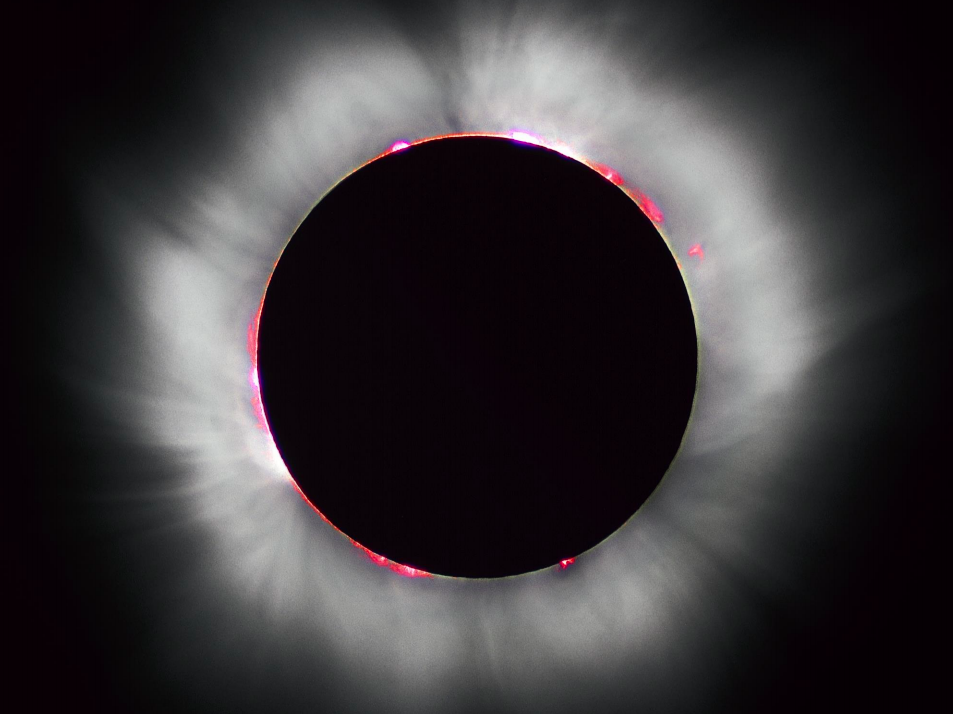
\includegraphics[width=0.5\textwidth]{poglavlja/7/slike/slika1.png}
\end{center}
\caption{Prikaz korona virusa}
\label{fig:pkv}
\end{figure}
\fi 
\section{Transformacija matrice rastojanja u evolutivno stablo}
\label{sec:transformacijamatrice}

Govorili smo o različitim vrstama poravnanja, između ostalog i o višestrukom poravnanju. Sada nećemo da ulazimo u to kako smo došli do višestrukog poravnanja, pretpostavimo samo da ga imamo. 

\subsection{Konstrukcija matrice rastojanja}
\label{subsec:matricarastojanja}

Na osnovu vi\v{s}estrukog poravnanja dobijamo matricu rastojanja iz koje \v{z}elimo da konstrui\v{s}emo evolutivno stablo. Defini\v{s}imo najpre \v{s}ta predstavlja svaki element ove matrice. Svaka kolona i svakak vrssta odgovara jednoj vrsti. Na glavnoj dijagonali su nule, a ostali elementi matrice označavaju broj različitih simbola u višestrukom poravnanju genoma dve vrste. Matrica je simetrična. Na slici \ref{fig:pkmr} možemo videti jedan primer matrice rastojanja. 

\begin{definicija}
Jedan element matrice u oznaci $D_{i,j}$ predstavlja broj razli\v{c}itih simbola u \textit{i}-tom i \textit{j}-tom redu vi\v{s}estrukog poravnanja.
\end{definicija}

\begin{figure}[h!]
\begin{center}
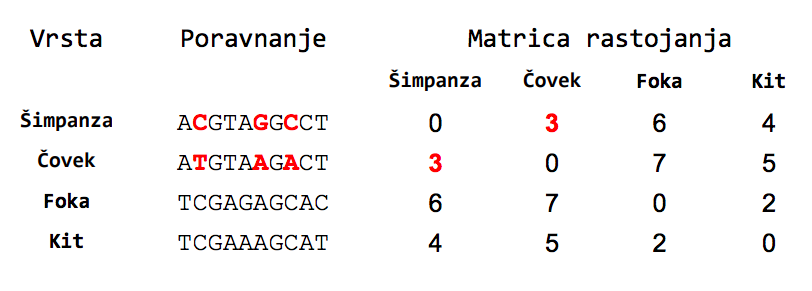
\includegraphics[width=0.75\textwidth]{poglavlja/7/slike/slika2.png}
\end{center}
\caption{Prikaz konstrukcije matrice rastojanja}
\label{fig:pkmr}
\end{figure}

Kada se radi filogenetska analiza obično se uzima protein za koji se zna da obavlja funkciju koja je izuzetno važna i koja se neće menjati tokom ogromnog broja godina. Takav protein se bira jer je on najviše konzerviran odnosno, u njemu se desilo najmanje mutacija. 

Za sve vrste korona virusa važi da se sastoje od 6 proteina, i od svih tih proteina odabran je tzv. \textit{spike} protein. 

\subsection{Stabla}
\label{subsec:stabla}

Dakle, biramo spike protein ovih vrsta, zatim konstruišemo matricu rastojanja na osnovu koje ćemo formirati evolutivno stablo.


Stablo je povezani acikli\v{c}ni graf. Za povezana acikli\v{c}na stabla se mo\v{z}e pokazati da svako stablo sa bar dva \v{c}vora sadr\v{z}i bar dva lista i svako stablo sa $n$ \v{c}vorova sadr\v{z}i ta\v{c}no $n - 1$ grana.


U evolutivnom stablu listovi predstavljaju dana\v{s}nje vrste (i oni su stepena 1)	, dok unutra\v{s}nji \v{c}vorovi predstavljaju izumrle vrste (stepena većeg od 1). Koreni \v{c}vor predstavlja najdaljeg zajedni\v{c}kog predaka. Koreni čvor predstavlja najdaljeg zajedničkog pretka. Od njega su sve ostale vrste potekle.

\begin{tcolorbox}
	\textbf{Problem filogeneze na osnovu rastojanja:} Konstruisatio evolutivno stablo na osnovu matrice rastojanja. \\
	\textbf{Ulaz:} Matrica rastojanja. \\
	\textbf{Izlaz:} Nekoreno stablo koje odgovara matrici rastojanja. 
\end{tcolorbox}

Na slici \ref{fig:pmrioes} se mo\v{z}e videti primer evolutivnog stabla koji odgovara matrici. Na koji način stablo odgovara matrici? Hajde da vidimo za čoveka i šimpanzu, vidimo da je cena puta od jednog do drugog jednaka 3, a ista ta vrednost upisana je u matricu. To važi i za sve ostale listove. Može se pojaviti grana težine 0. Ukoliko se to desi između unutrašnjih čvorova, oni se spajaju. Međutim, u našem primeru to se desilo između unutrašnjeg čvora i lista. Ako bismo ih spojili to bi značilo da je kit izumrela vrsta. 


\begin{figure}[h!]
\begin{center}
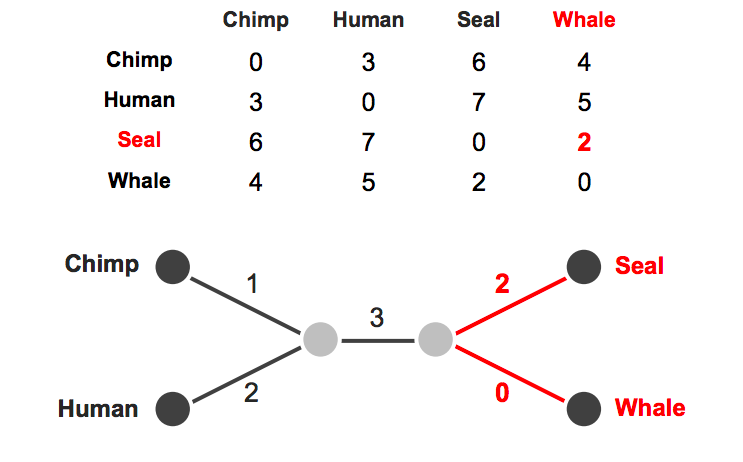
\includegraphics[width=0.75\textwidth]{poglavlja/7/slike/slika3.png}
\end{center}
\caption{Prikaz matrice rastojanja i njenog odgovaraju\'ceg evolutivnog stabla}
\label{fig:pmrioes}
\end{figure}


Uvodimo pojam rastojanja izme\dj u dva lista \textit{i} i \textit{j} u evolutivnom stablu u oznaci $d_{i, j}$.
\begin{tcolorbox}
\textbf{Problem izra\v{c}unavanja rastojanja izme\dj u listova:} Za dato te\v{z}insko stablo, izra\v{c}unati rastojanje izme\dj u listova.\\
\textbf{Ulaz}: Te\v{z}insko stablo sa n listova.\\
\textbf{Izlaz}: Matrica n x n ($d_{i, j}$), gde je $d_{i, j}$ du\v{z}ina putanje izme\dj u listova \textit{i} i \textit{j}.
\end{tcolorbox}

Ovaj problem jeste lako re\v{s}iv, međutim, zanima nas kako da za datu matricu rastojanja konstrui\v{s}emo evolutivno stablo. S obzirom na to da je mogu\'ce da iz jedne matrice dobijemo vi\v{s}e razli\v{c}itih stabala, neophodno je da matrice zadovoljavaju odre\dj ena svojstva, kako bi za jednu matricu dobili ta\v{c}no jedno stablo. Da bi to bilo mogu\'ce matrica mora biti aditivna. 

\begin{definicija}
Za dato evolutivno stablo, matricu koja opisuje rastojanja izme\dj u njegovih listova zovemo \textit{aditivnom matricom}
\end{definicija}

\begin{teorema}
Matrica \textit{D} je aditivna akko za proizvoljna \v{c}etiri indeksa u matrici \textit{i, j} i \textit{k, l} va\v{z}i:

\begin{center}
\textit{$D_{ij}$ + $D_{kl}$ \textless= $D_{ik}$+$D_{jl}$ = $D_{il}$ + $D_{jk}$}
\end{center}

\end{teorema}

Na osnovu ove teoreme i definicije mo\v{z}emo zaklju\v{c}iti na koji na\v{c}in da pove\v{z}emo listove u evolutivnom stablu \ref{fig:pples}.

\begin{figure}[h!]
\begin{center}
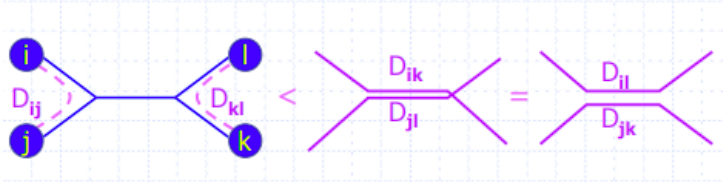
\includegraphics[width=0.75\textwidth]{poglavlja/7/slike/slika4.png}
\end{center}
\caption{Prikaz povezivanja listova u evolutivnom stablu}
\label{fig:pples}
\end{figure}

Po\v{s}to je za jednu matricu mogu\'ce konstruisati vi\v{s}e evolutivnih stabala, uvek je bolje izabrati prosto stablo. 

\begin{definicija}
\textbf{Prosto stablo:} stablo bez \v{c}vorova stepena 2.
\end{definicija}

\begin{teorema}
Postoji ta\v{c}no jedno prosto stablo koje odgovara aditivnoj matrici.
\end{teorema}

Sada mo\v{z}emo formulisati \textbf{problem filogeneze na osnovu rastojanja}:

\begin{tcolorbox}
\textbf{Problem filogeneze na osnovu rastojanja:}
Konstruisati evolutivno stablo na osnovu aditivne matrice rastojanja. \\
\textbf{Ulaz:} Aditivna matrica rastojanja.\\
\textbf{Izlaz:} Prosto stablo koje odgovara datoj matrici rastojanja.
\end{tcolorbox}

\section{Prema algoritmu za rekonstrukciju filogenetskog stabla na osnovu rastojanja}
\label{pazrfsnor}

Primetimo da minimalna pozitivna vrednost matrice rastojanja odgovara listovima u stablu koje povezuje zajedni\v{c}ki roditelj. Takve listove nazivamo \textbf{susednim listovima}. Susedni listovi imaju zajedničkog pretka. U primeru \ref{fig:pmrioes} foka i kit su susedi (jer dele istog roditelja). Šta ako ne postoje susedni listovi u stablu? Sledeća teorema nam pomaže:

\begin{teorema}
	Za svako prosto stablo sa bar dva \v{c}vora postoji bar jedan par susednih listova.
\end{teorema}

\iffalse 
\begin{figure}[h!]
\begin{center}
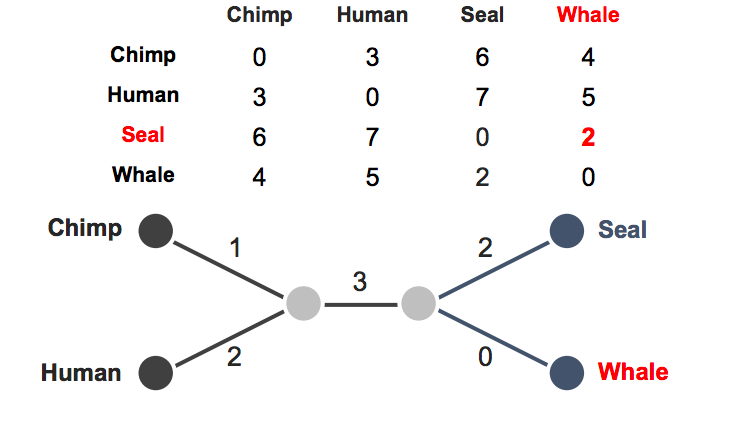
\includegraphics[width=0.75\textwidth]{poglavlja/7/slike/slika5.png}
\end{center}
\caption{Prikaz susednih listova}
\label{fig:psl}
\end{figure}
\fi 

Dakle, mo\v{z}emo pretpostaviti da \'cemo uvek imati par susednih listova. Mi znamo da su \textit{kit} i \textit{foka} susedni listovi i da dele zajedni\v{c}kog roditelja, me\dj utim, ne znamo koja se vrednost pridru\v{z}uje svakoj od ovih grana. Da bismo dobili rastojanje izme\dj u susednih listova \textit{i} i \textit{j} od roditelja \textit{m} potrebno je da imamo jo\v{s} neki list unutar takvog stabla, recimo list \textit{k}. Razmatramo slede\'ca rastojanja: $d_{i,k}, d_{j, k}, d_{i,j}$ su rastojanja izme\dj u listova koja su data u matrici rastojanja, dok rastojanja $d_{i, m}$ i $d_{j, m}$ koja predstavljaju rastojanja izme\dj u lista i unutra\v{s}njeg \v{c}vora, nisu data \ref{fig:filstab}.

Da bismo dobili rastojanje izme\dj u \v{c}ora \textit{i} i \v{c}vora \textit{j} treba da pratimo ljubi\v{c}asto i plavo rastojanje \ref{fig:filstab}. Sli\v{c}no ra\v{c}unamo i $d_{i, k}$ i $d_{j, k}$, a $d_{k, m}$ dobijamo sabiranjem kao na slici \ref{fig:filstab}. Sa velikim \textbf{D} ($D_{i, k}, D_{j, k}, D_{i, j}$) ozna\v{c}avamo elemente matrice rastojanja, dok sa malim \textbf{d} ozna\v{c}avamo rastojanje izme\dj u bilo koja dva \v{c}ora u evolutivnom stablu. 

Kada znamo rastojanje od $d_{k,m}$ sada mo\v{z}emo da dobijemo $d_{i,m}$ kao: ($D_{i, k} + D_{i, j} – D_{j, k}$) / 2. Analogno dobijamo i za drugog suseda $d_{j, m}$. Obratimo pa\v{z}nju da je \v{c}vor \textit{k} proizvoljan - bilo koji list koji je razli\v{c}it od listova \v{c}ija rastojanja do roditeljskog \v{c}vora tra\v{z}imo.

\begin{figure}[h!]
\begin{center}
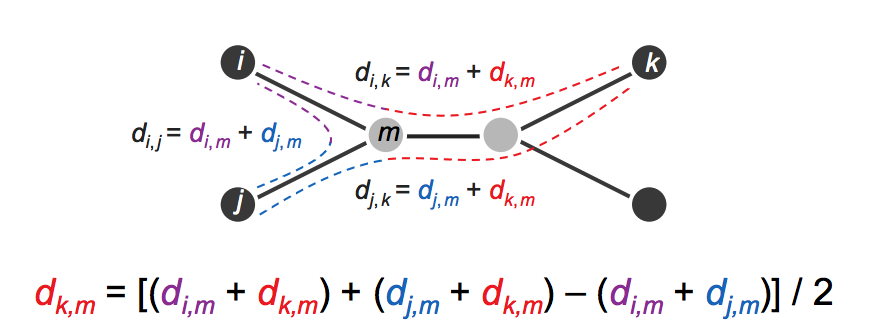
\includegraphics[width=0.7\textwidth]{poglavlja/7/slike/slika7.png}
\end{center}
\caption{Prikaz rekonstrukcije filogenetskog stabla na osnovu rastojanja}
\label{fig:filstab}
\end{figure}

Formula za rastojanje $d_{k, m}$, data na slici \ref{fig:filstab}, nije nam pogodna jer zavisi od čvora $m$. Čvor $m$ je unutrašnji čvor i za njega nemamo rastojanja u matrici. Zbog toga prezapisujemo formulu na sledeći način:

$$d_{k, m} = (d_{i, k} + d_{j, k} - d_{i, j}) / 2 = (D_{i, k} + D_{j, k} - D_{i, j}) / 2$$
 
Sada su nam sva rastojanja poznata, odnosno koristimo samo rastojanja između listova. To znači da vrednost između lista i unutrašnjeg čvora možemo da izračunamo preko listova. Na ovaj način, kada znamo rastojanje između $k$ i $m$, možemo i da izračunamo rastojanje od $i$ do $m$, sledećom formulom:

$$d_{i, m} = D_{i, k} - (D_{i, k} + D_{j, k} - D_{i, j}) / 2 = (D_{i, k} + D_{i, j} - D_{j, k}) / 2  $$

Obratimo pažnju da je $k$ proizvoljan čvor. Uzeli smo bilo koji list koji je bio različit od susednih lvorova $i$ i $j$.

Posmatrajmo sada opet evolutivno stablo. Foka \'ce biti \v{c}vor \textit{i}, \textit{j} \'ce biti susedan \v{c}vor kit. Za \textit{k} mo\v{z}emo uzeti po algoritmu, bilo koji \v{c}vor, biramo \v{s}impanzu. Sada va\v{z}i: 
\begin{center}
$d_{Seal, m} = (D_{Seal, Chimp} + D_{Seal, Whale} – D_{Whale, Chimp}) / 2 = 2$
\end{center}

Kada smo odredili vrednost grane od foke do unutrašnjeg čvora, treba da odredimo i vrednost od unutrašnjeg čvora do kita. To je lako jer znamo ukupno rastojanje od foke do kita, koje iznosi 2, i upravo smo odredili rastojanje od foke do unutrašnjeg čvora, koje takođe iznosi 2. Zbog toga, rastojanje od unutrašnjeg čvora do kita mora biti 0. 

Kada su određene ove vrednosti, uvodimo novu vrstu i kolonu u matricu za čvor $m$. Ona sadrži rastojanja do listova kit i foka. Sada u matrici više ne gledamo kita i foku, već gledamo samo čvor $m$ i računamo ostala rastojanja. Smanjili smo matricu rastojanja na tri vrste, kao na slici \ref{fig:mala}. Dalje ponavljamo postupak. 


\begin{minipage}{\textwidth}
	\centering
	\begin{minipage}{0.45\textwidth}
		\begin{figure}[H]
			\centering
			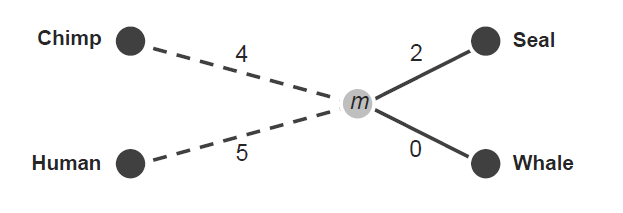
\includegraphics[width=\textwidth]{poglavlja/7/slike/humanChimp.png}
			\caption{Vrednosti za Seal i Whale su određene i više ih ne koristimo.}
			\label{slika:rekurzivno}
		\end{figure} 
	\end{minipage}
	\hfill 
	\begin{minipage}{0.45\textwidth}
		\begin{figure}[H]
			\centering
			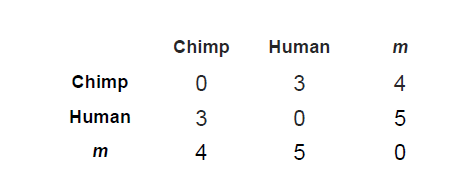
\includegraphics[width=\textwidth]{poglavlja/7/slike/malaMatrica.png}
			\caption{Uveden je novi čvor $m$ koji posmatramo umesto Seal i Whale.}
			\label{fig:mala}
		\end{figure}  
	\end{minipage}
	\vspace*{1em}
\end{minipage}


Ovakav rekurzivni pristup nije moguce primeniti za svaku matricu. U tim situacijama koristimo \textit{AdditivePhylogeny} algoritam.

\section{AdditivePhylogeny algoritam}
\label{addalg}

\begin{figure}[h!]
\begin{center}
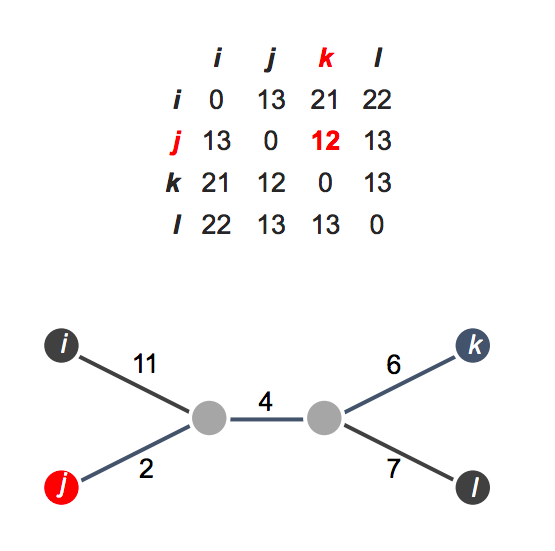
\includegraphics[width=0.5\textwidth]{poglavlja/7/slike/slika6.png}
\end{center}
\caption{Primer matrice za koju ne mo\v{z}emo primeniti prethodni pristup}
\label{fig:pmzknppp}
\end{figure}

Na slici \ref{fig:pmzknppp} prikazana je matrica za koju ne možemo da primenimo rekurzivni algoritam. Problem je što ćemo u nekom trenutku dobiti granu koja ima negativnu vrendost. Zašto algoritam ne radi? Mo\v{z}emo videti da je minimalni element $D_{j,k}$, a \textit{j} i \textit{k} nisu susedi, zato ne mo\v{z}emo primeniti prethodni pristup, iako je matrica ultrametri\v{c}na. Međutim, ova matrica ima odgovarajuće stablo i ono je prikazano na slici \ref{fig:pmzknppp}. Umesto tra\v{z}enja suseda, poku\v{s}ajmo da izra\v{c}unamo du\v{z}inu krajnjih grana, onih grana koje vode do listova. Formule iz rekurzivnog algoritma (slika \ref{fig:filstab}) važe ako su $i$ i $j$ susedni čvorovi. Ovde će važiti slična formula, a sledeća teorema nam govori tome:

\begin{teorema}
	\label{teorem:limb}
\textbf{O du\v{z}ini spoljnih grana:} \textit{LimbLength(i)} je jednako minimalnoj vrednosti ($D_{i, k}$ + $D_{i, j}$ - $D_{j, k}$)/2 po svim listovima \textit{j} i \textit{k}.
\end{teorema}

Isklju\v{c}ujemo pretpostavku koju smo imali kod susednih listova, dakle ra\v{c}unamo rastojanje samo za jedan list, jer ne znamo koji joj je susedni \v{c}vor, pa zato uzimamo sve kombinacije za \textit{j} i \textit{k}. 
\\
\\
\noindent Prika\v{z}imo AdditivePhylogeny algoritam:

\begin{enumerate}
	\item Izaberemo proizvoljno list, npr. \textit{j}. 
	\item Izra\v{c}unamo du\v{z}inu njegove krajnje grane, LimbLength(\textit{j}). Uzećemo sve moguće kombinacije za preostala dva čvora ($i$ i $k$, $i$ i $l$, $k$ i $l$) i izračunaćemo minimum. Tako dobijemo vrednost 2.
	\item Oduzmemo $LimbLength(\textit{j})$ od svake grane i dobijemo matricu \textit{$D^{bald}$}  u kojoj do lista \textit{j} vodi ogoljena (bold) grana (du\v{z}ine 0). Dakle, $j$-toj vrsti i $j$-toj koloni umanjujemo vrednosti za $LimbLength(\textit{j})$. Stanje nakon promene prikazano je na slici \ref{dbald}.   
	\item Uklonimo \textit{j}-ti red i kolonu iz matrice i dobijemo $(n - 1) \times (n - 1)$ matricu \textit{$D^{trim}$}. 
	\item  Konstrui\v{s}emo Tree($D^{trim}$) - rekurzivno. 
	\item Identifikujemo ta\v{c}ku u Tree($D^{trim}$) gde list \textit{j} treba da se nalazi. Ovom koraku ćemo se posebno posvetiti. 
	\item  Dodamo list \textit{j} povezujuci ga granom du\v{z}ine LimbLength(\textit{j}) kako bismo formirali Tree(\textit{D}). 
\end{enumerate}


\begin{figure}[h!]
	\begin{center}
		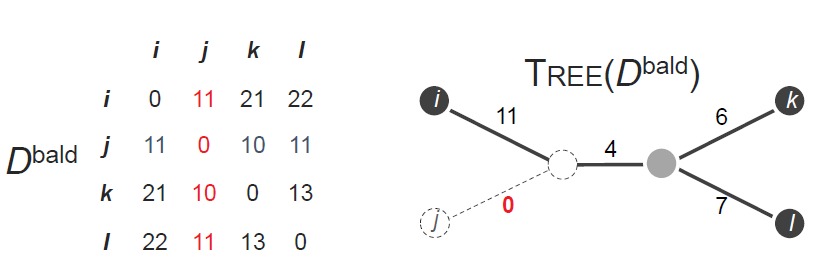
\includegraphics[width=0.8\textwidth]{poglavlja/7/slike/Dbold.png}
	\end{center}
	\caption{Izgled matrice i stabla nakon umanjivanja vrednosti za $LimbLength(\textit{j})$}
	\label{dbald}
\end{figure}

Ta\v{c}ku povezivanja za list \textit{j} odredićemo na osnovu teoreme \ref{teorem:limb}.  Tačka treba da se nađe na putanji izme\dj u listova \textit{i} i \textit{k} na rastojanju $D^{bald}_{i, j}$ od \textit{i}. Dakle va\v{z}i: $D^{bald}_{i, j} + D^{bald}_{j, k} = D^{bald}_{i, k}$. Kada smo pronašli tačku treba dodati čvor $j$. Prvo grana koja je povezivala čvor $i$ sa unutrašnjim čvorom (označimo ga sa $u$) mora da se ukloni. Zatim se dodaje novi unutrašnji čvor (označimo ga sa $m$) na koji se povezuju $i$ i $j$. Trenutno smo u $D^{bald}$ stablu pa je dužina od $j$ do $m$ jednaka 0, a dužina od $i$ do $m$ jednaka je $D^{bald}_{i, j}$. Dužina od $m$ do drugog unutrašnjeg čvora iznosi $D^{trim}_{i, u} - D^{bald}_{i, m}$. Prikaz postupka može se videti na slikama \ref{slika:dtrim} i \ref{fig:dbald}.



\begin{minipage}{\textwidth}
	\centering
	\begin{minipage}{0.45\textwidth}
		\begin{figure}[H]
			\centering
			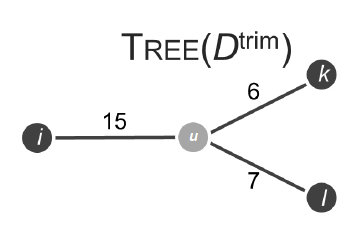
\includegraphics[width=\textwidth]{poglavlja/7/slike/Dtrim.png}
			\caption{Tražimo tačku gde treba da umetnemo čvor $j$.}
			\label{slika:dtrim}
		\end{figure} 
	\end{minipage}
	\hfill 
	\begin{minipage}{0.45\textwidth}
		\begin{figure}[H]
			\centering
			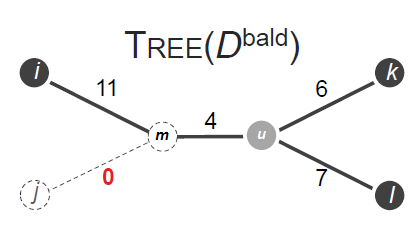
\includegraphics[width=\textwidth]{poglavlja/7/slike/Dbald.png}
			\caption{Dodajemo čvor $j$ u stablo.}
			\label{fig:dbald}
		\end{figure}  
	\end{minipage}
	\vspace*{1em}
\end{minipage}


Dobra strana ovog algoritma je da kreira stablo koje odgovara aditivnoj matrici, a lo\v{s}a da ne radi za neaditivne matrice.
 
\section{Metod najmanjih kvadrata}
\label{sec:metodnajmanjihkvadrata}

U slu\v{c}aju da matrica nije aditivna, treba je aproksimirati nekom aditivnom matricom. Na slici \ref{fig:lsq} prikazana je jedna neaditivna matrica ($D$) za stablo $T$. Matrica $d$ je njena aproksimacija koju je, u ovom slučaju, bilo lako odrediti. Samo smo izmenili crvene vrednosti. Šta se radi u komplikovanijemo slučaju? Računamo diskrepancu za stablo $T$ i odgovarajuću matricu $D$:

\begin{figure}[h!]
	\centering
	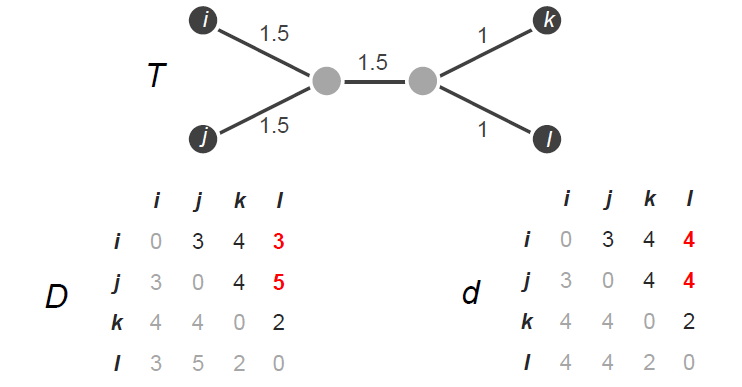
\includegraphics[width=0.8\textwidth]{poglavlja/7/slike/metodNajmanjihKvadrata.png}
	\caption{Matrica $D$ nije aditivna i ne možemo primeniti prethodni algoritam. Možemo je aproksimirati aditivnom matricom.}
	\label{fig:lsq}
\end{figure}

$$Discrepancy(T, D) = \sum_{1 \leq i \textless j \leq n} (d_{i, j}(T) - D_{i, j})^{2}$$

Diskrepanca određuje koliko je $d$ dobra aproksimacija za $D$. U ovom slučaju matrica $d$ nam je bila poznata. Šta da radimo ako nemamo aditivnu matricu? Treba dodeliti du\v{z}ine granama u stablu T tako da veli\v{c}ina Discrepancy(T, D) bude minimalna.

U op\v{s}tem slu\v{c}aju, za stablo date topologije postoji algoritam polinomijalne slo\v{z}enosti koji \'ce dodeliti du\v{z}ine granama stabla tako da diskrepanca bude minimalna. Me\dj utim, u prakti\v{c}nim primenama ne\'ce biti poznata topologija stabla pa stoga moramo ra\v{c}unati minimum po svim mogu\'cim stablima. Sa dodavanjem svakog lista u stablo, broj razli\v{c}itih topologija stabala raste eksponencijalno. Problem minimizacije diskrepance po svim mogu\'cim stablima je NP kompletan. U nastavku, razmotri\'cemo dve heuristike za konstrukciju stabla na osnovu neaditivnih matrica.

Prva heuristika tiče se posebne vrste stabala, a to su ultrametrična evolutvna stabla. Pre nego što ih opišemo prvi da se upoznamo sa još nekim pojmovima.


\subsection{Modelovanje specijacije}
\label{subsec:ms}

U prakti\v{c}nim primenama, istra\v{z}iva\v{c}i \v{c}esto pretpostavljaju da svaki unutra\v{s}nji \v{c}vor odgovara \textit{specijaciji} kada se jedna vrsta deli na dve. Podsetimo se da u listovima se nalaze organizmi koje pripadaju vrste koje postoje danas, a u unutrašnjim čvorovima su izumrele vrste. Čvor koji ima dva potomka odgovara evolutivnom događaju specijacije kada je jedna vrsta izumrela ali su sve dve vrste tada razdvojile.

\begin{definicija}
\textbf{Nekoreno binarno stablo:} svaki \v{c}vor je stepena 1 ili 3.
\end{definicija}

\begin{definicija}
\textbf{Koreno binarno stablo:} nekoreno binarno stablo sa korenom (jedini će biti stepena 2) postavljenom na jednoj od grana.
\end{definicija}

\subsection{Ultrametri\v{c}na stabla}
\label{subsec:us}

Recimo da smo odredili korensko stablo. Sada želimo da svakom čvoru dodelimo startost. Listovi imaju starost 0 (starost u smislu pre koliko miliona godina su izumrele).


\begin{definicija}
\textbf{Molekularni sat:} dodeljuje starost svakom \v{c}voru u stablu (starost listova = 0).
\end{definicija}

\begin{definicija}
\textbf{Te\v{z}ine grana:} razlika u starosti \v{c}vorova koje povezuju.
\end{definicija}

\begin{definicija}
\textbf{Ultrametri\v{c}no stablo:} koreno stablo u kom važi da udaljenost od korena do bilo kog lista je ista i predstavlja starost korena.
\end{definicija}

\noindent\textbf{UPGMA: heuristi\v{c}ko klasterovanje}
\label{subsec:upgma}

\begin{enumerate}
\item Formirati klaster za svaku dana\v{s}nju vrstu. Svaki klaster sadr\v{z}i jedan list.
\item Na\'ci dva najbli\v{z}a klastera $C_1$ i $C_2$ na osnovu prose\v{c}nog rastojanja izme\dj u njihovih \v{c}lanova $D_{avg}(C_1, C_2)$ = $\sum_{i\ in\ C_1, j\ in\ C_2} D_{i, j} / \mid C_1 \mid \bullet \mid C_2 \mid $ gde $\mid C \mid$ ozna\v{c}ava broj elemenata u klasteru C. Za jednočlane klastere rastojanje je dato u matrici rastojanja.
\item Spojiti $C_1$ i $C_2$ u jedinstveni klaster C.
\item Formirati novi \v{c}vor za klaster i granama povezati ga za \v{c}vorovima. Postaviti starost \v{c}vora C na $D_{avg}$($C_1$, $C_2$)/2.
\item A\v{z}urirati matricu rastojanja tako \v{s}to ubacimo novi \v{c}vor, izbacimo \v{c}vorove koje on sadr\v{z}i i izra\v{c}unamo rastojanja kao prose\v{c}na rastojanja izme\dj u svaka dva para klastera.
\item Iteriramo dok ne do\dj emo do jednog klastera koji sadr\v{z}i sve vrste.
\end{enumerate}

Dobra strana ovog algoritma je da kreira stablo za svaku matricu, a lo\v{s}a da stablo ne mora da odgovara aditivnoj matrici. Na slici \ref{upgma} je prikazan primer stabla dobijen ovim algoritmom. Vidimo da stablo ne odnovara datoj aditivnoj matrici.

\begin{figure}[h!]
	\centering
	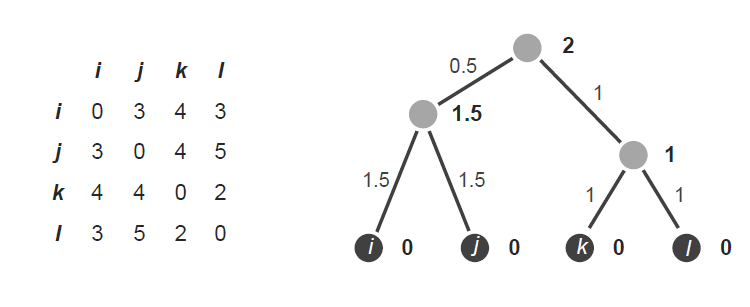
\includegraphics[width=0.8\textwidth]{poglavlja/7/slike/upgma.png}
	\caption{Stablo dobijeno primenom heuristike UPGMA.}
	\label{upgma}
\end{figure}


\section{Neighbour-Joining teorema}
\label{sec:njt}

Za datu matricu rastojanja \textit{D} dimenzije \textit{n x n}, njena \textbf{neighbour-joining} matrica u oznaci \textit{D*} defini\v{s}e se kao:\\

$$D^*_{i, j} = (n - 2) \bullet D_{i, j} - TotalDistance_D(i) - TotalDistance_D(j)$$


 gde je $TotalDistance_D(i)$ suma rastojanja od \textit{i} do svih ostalih listova.

\begin{teorema}
\textbf{Neighbour-joining:} ako je matrica \textit{D} aditivna, onda minimalni element matrice \textit{D*} odgovara susednim listovima u stablu \textit{Tree(D)}.
\end{teorema}

\begin{enumerate}
\item Konstrui\v{s}emo neighbour-joining matricu D* na osnovu matrice D.
\item Na\dj emo minimalni element $D^*_{i, j}$ matrice D*.
\item Izra\v{c}unamo $\bigtriangleup_{i, j} = (TotalDistance_d(i) - TotalDistance_d(j)) / (n - 2)$.
\item Našli smo da $i$ i $j$ imaju zajedničkog pretka i povezujemo ih u jedan čvor. Treba da odredimo težine grana do novog čvora. Postavimo $LimbLength(i)$ na $1/2(D_{i, j} + \bigtriangleup_{i, j})$ i $LimbLength(j)$ na $1/2(D_{i, j} + \bigtriangleup_{i, j})$.
\item Formiramo matricu D' tako \v{s}to uklonimo \textit{i}-ti i \textit{j}-ti red/kolonu iz D i dodamo \textit{m}-ti red/kolonu tako da za svako k va\v{z}i $D_{k, m}$ = ($D_{i, k} + D_{j, k} - D_{i, j}$) / 2. Ovim smo smanjili dimenziju našeg problema za 1.
\item Primenimo \textit{NeighborJoining} rekurzivno na D' da dobijemo Tree(D').
\item Vratimo krajnje grane do \v{c}vorova \textit{i} i \textit{j} i dobijemo Tree(D).
\end{enumerate}

Iako je \textit{Neighbor Joining} algoritam bio revolucionarno otkriće. Međutim, metodi zasnovani na rastojanju imaju i mane. Dakle, mi smo birali nekakve reprezentativne sekvence, zatim smo ih poravnali. Kada vi\v{s}estruko poravnanje zamenimo matricom rastojanja, gubimo informacije o sekvencama iz poravnanja. Zbog toga ne mo\v{z}emo da zaklju\v{c}imo kakva je sekvenca odgovarala vrstama iz unutra\v{s}njih \v{c}vorova. Samim tim ne možemo da vidimo do kakvih je to mutacija tačno došlo tokom evolucije.



\section{Rekonstrukcija stabla na osnovu karakteristika}
\label{sec:rsnok}

Pre oko pedeset godina, istra\v{z}iva\v{c}i su konstruisali filogenetska stabla na osnovu anatomsko-fiziolo\v{s}kih osobina organizama koje su nazvane \textbf{karakteristikama}. U odnosu na karakteristike konstruisali su tabele karakteristika. Jedna takva tabela prikazana je na slici  \ref{fig:karak}. One koji imaju slične karakteristike smatramo bližim evolutivnim rođacima.

\begin{figure}[h!]
\begin{center}
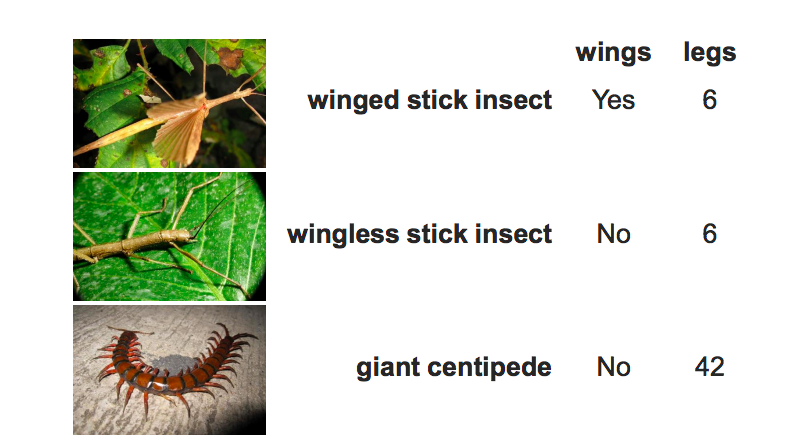
\includegraphics[width=0.7\textwidth]{poglavlja/7/slike/slika10.png}
\caption{Tabela karakteristika}
\label{fig:karak}
\end{center}
\end{figure}

Ono što bi mogao da bude problem jeste to što se mi u ovom poglavlju bavimo virusima. Za njih baš nemamo tako očigledne karakteristike, kao što su ima/nema krila, broj nogu i slično. Ovako nešto nije primenjivo na njih.

\subsection{Filogeneza na osnovu karakteristika}
\label{subsec:fnok}

\begin{tcolorbox}
\textbf{Problem filogeneze zasnovane na karakteristikama:} Rekonstruisati evolutivno stablo na osnovu karakteristika. \\
Ulaz: Tabela karakteristika n x m za n vrsta i m karakteristika. \\
Izlaz: Stablo kog kog su vrste sa sli\v{c}nim karakteristikama blizu jedna drugoj. 
\end{tcolorbox}

Kako bismo konstruisali evolutivno stablo na osnovu karakteristika? Ako bismo radili sa insektima, na jednu stranu bismo stavili one koji npr. imaju krila, a sa druge one koji nemaju krila.

\textbf{Doloov zakon o nepovratnosti evolucionih procesa (1893):} \textit{evolucija ne izmi\v{s}lja dva puta isti organ (npr. krila kod insekata).}

Ipak, pojavili su se izuzeci Doloovog zakona. Ispitivanje je rađeno na velikom uzorku insekata. Tokom studije pronađen je izuzetak Doloovog zakona, desilo se da je vrsta izgubila krila tokom evolucije, a kasnije tokom evolucije krila su se ponovo razvila. Kako je to moguće?

Vratimo se na DNK, na osnovu svega. Unutar DNK je upisano kako će izgledati svaki organ koji neki organizam poseduje. To što je nešto zapisano u okviru DNK ne znači da će se to ispoljiti. Tako kod insekata, jedna vrsta možda sadrži gen za krila, ali on se ne mora ispoljiti baš kod te vrste, može i kod nekog njenog potomka. Do ekspresije može, i ne mora da dođe. 


Došlo se do ideje da se poravnanje koristi kao tabela karakteristika (poravnanje DNK ili RNK sekvenci). Tako bismo rešili problem karakteristika kod virusa.

\section{Problem male parsimonije}
\label{sec:pmp}

Dato nam je binarno stablo. U listovima su organizmi. Ono što nas zanima jesu sekvence predaka. Na slici \ref{slika:malaParsimonija} data nam je tabela karakteristika i stablo. Ono što je poznato jeste koji su listovi susedni. Zanima nas do kakvih je mutacija došlo tokom evolucije, odnosno, zanima nas koja je sekvenca njihovog zajedničkog pretka. 

\begin{minipage}{\textwidth}
	\centering
	\begin{minipage}{0.45\textwidth}
		\begin{figure}[H]
			\centering
			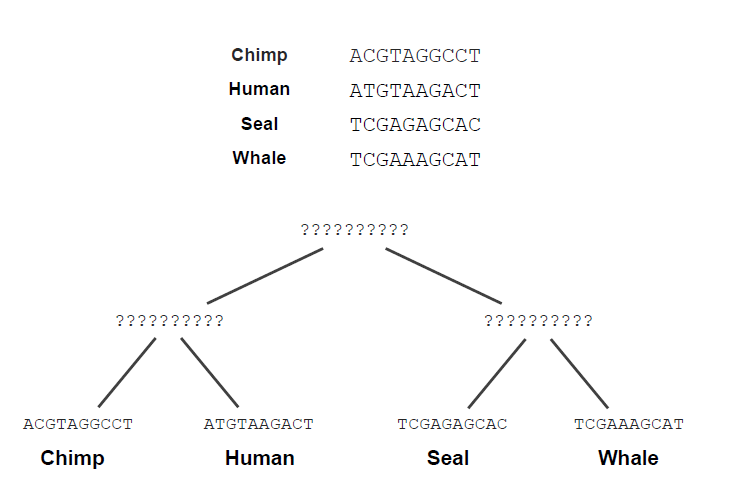
\includegraphics[width=\textwidth]{poglavlja/7/slike/malaParsemonija.png}
			\caption{U listovima su sekvence različitih vrsta i želimo da otkrijemo sekvence njihovih predaka.}
			\label{slika:malaParsimonija}
		\end{figure} 
	\end{minipage}
	\hfill 
	\begin{minipage}{0.45\textwidth}
		\begin{figure}[H]
			\centering
			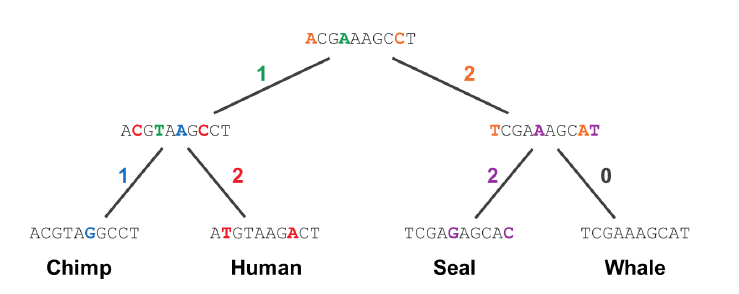
\includegraphics[width=\textwidth]{poglavlja/7/slike/malaParsemonija2.png}
			\caption{Skor parsimonije}
			\label{slika:malaParsimonijaSkor}
		\end{figure}  
	\end{minipage}
	\vspace*{1em}
\end{minipage}

Na slici \ref{slika:malaParsimonijaSkor} dato je jedno moguće rešenje. Kvalitete rešenja određuje nam skor. Skor parsimonije je suma Hamingovih rastojanja du\v{z} svake grane. Za svaku granu možemo da odredimo Hamingovo rastojanje niski koje se nalaze na krajevima te grane. Skor parsimonije na ovoj slici jednak je 8.

\begin{tcolorbox}
\textbf{Problem male parsimonije:} Odrediti oznake za unutra\v{s}nje \v{c}vorove korenog stabla. \\
Ulaz: Koreno binarno stablo gde je svaki list ozna\v{c}en jednim simbolom.\\
Izlaz: Oznake za sve ostale \v{c}vorove stabla takve da minimizuju skor parsimonije stabla.
\end{tcolorbox}


Algoritam dinami\v{c}kog programiranja: Neka je $T_v$ podstablo stabla T sa korenom u \v{c}voru v. Neka je $s_k(v)$ minimalni skor parsimonije stabla $T_v$ za sva mogu\'ca obele\v{z}avanja, pod pretpostavkom da je \v{c}vor v obele\v{z}en simbolom k. Minimalni skor parsimonije stabla jednak je minimalnoj vrednosti $s_k(root)$ po svim simbolima k. Neka je \textit{$\delta_{i, j}$} Kronekerov delta simbol:
\begin{itemize}
\item \textit{$\delta_{i, j}$} = 0 ako i = j
\item \textit{$\delta_{i, j}$} = 1 ina\v{c}e
\end{itemize}
Va\v{z}i slede\'ca rekurentna relacija:

$$s_k(v) = min_{all\ symbols\ i} {s_i(Daughter(v)) + \delta_{i,k}} + min_{all\ symbols\ j} {s_j(Son(v)) + \delta_{j,k}}$$

\noindent gde $Daughter(v)$ označava levo podstablo, a $Son(v)$ desno podstablo sa korenom u čvoru $v$. 

Pogledajmo na primeru kako to funkcioniše. Na početku imamo po jedan nukleotid u svakom listu. Njegova vrednost je obeležena sa 0, dok je kod ostalih vrednost $\infty$. Onda za svaki nukelotid računamo skor parsimonije i uzimamo vrednost koja je minimalna. To radimo dok ne stignemo do korena. Kada stignemo do korena radimo backtraking, ondnosno idemo unazad kako bismo odredili oznake za unutrašnje čvorove. Biramo ih tako da bude što manje mutacija, a to je nukleotid kome odgovara najmanja vrednost. Može se desiti da više nukleotida ima najmanju vrednost i tada je u suštini sve jedno koji ćemo odabrati. Međutim, ako je neki od tih nukleotida predak najbolje je da njega odaberemo kako ne bi bilo mutacije. Na slici \ref{slika:dpMP} prikazan je jedan primer izvršavanja ovog algoritma.


\begin{figure}[h]
	\centering
	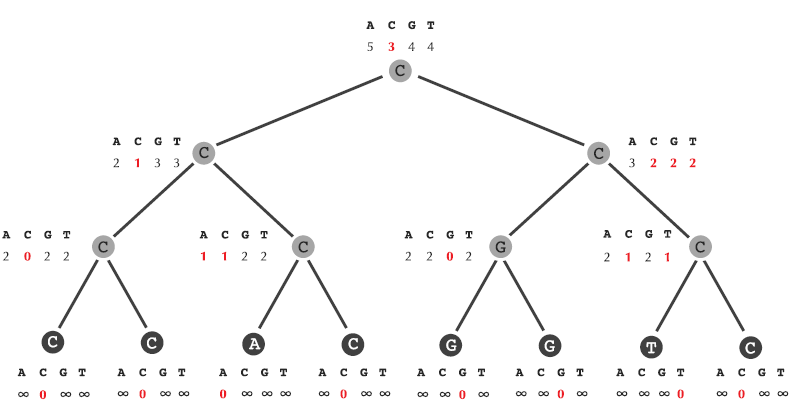
\includegraphics[width=\textwidth]{poglavlja/7/slike/dpMalaParsemonija.png}
	\caption{Primena algoritma dinamičkog programiranja na problem male parsimonije.}
	\label{slika:dpMP}
\end{figure}


\section{Problem velike parsimonije}
\label{sec:pvp}

Kod problema male parsimonije, filogenetska stabla su uvek binarna i uvek korena. Algoritam za rešavanje podrazumeva da nam je poznata topologija stabla, odnosno, znamo gde koji čvor stoji. Nekada to nije poznato, ne znamo koji listovi treba da budu susedni. Ovo je problem velike parsimonije i u nastavku ćemo ga detaljnije opisati.


\begin{tcolorbox}
\textbf{Problem velike parsimonije:} Za dati skup niski, na\'ci stablo \v{c}iji su listovi ozna\v{c}eni ovim niskama koje ima najmanji skor parsimonije. \\
Ulaz: Kolekcija niski jednake du\v{z}ine. \\
Izlaz: Koreno binarno stablo T koje minimizuje skor parsimonije po svim mogu\'cim korenim binarnim stablima \v{c}iji su listovi ozna\v{c}eni datim niskama.\\
Ovaj problem je NP-kompletan.
\end{tcolorbox}

\subsection{Pohlepna heuristika za veliku parsimoniju}
\label{phzvp}

Trenutno posmatramo nekoreno stablo, bitno je da ćemo lako odrediti koreno. Od celog stabla izdvojili smo jednu unustrašnju granu koja spaja unutrašnje čvorove $a$ i $b$ (sa po najviše 2 potomka). Svaki od ovih čvorova može imati dalje potomke pa definišemo četiri podstabla. Primetimo da uklanjanje unutra\v{s}nje grane od $a$ do $b$ (i oba čvora sa ostalim granama koje su povezane na njih) dovodi do stvaranja \v{c}etiri podstabla (W, X, Y, Z) \ref{fig:pscp}. 

Pre nego što smo uklonili ove grane, pretpostavili smo raspored kakav je na slici \ref{fig:pscp}. Dakle, pretpostavili smo neku topologiju. Međutim, to je nešto što nam nije poznato kod problema velike parsemonije.

\begin{figure}[h!]
\begin{center}
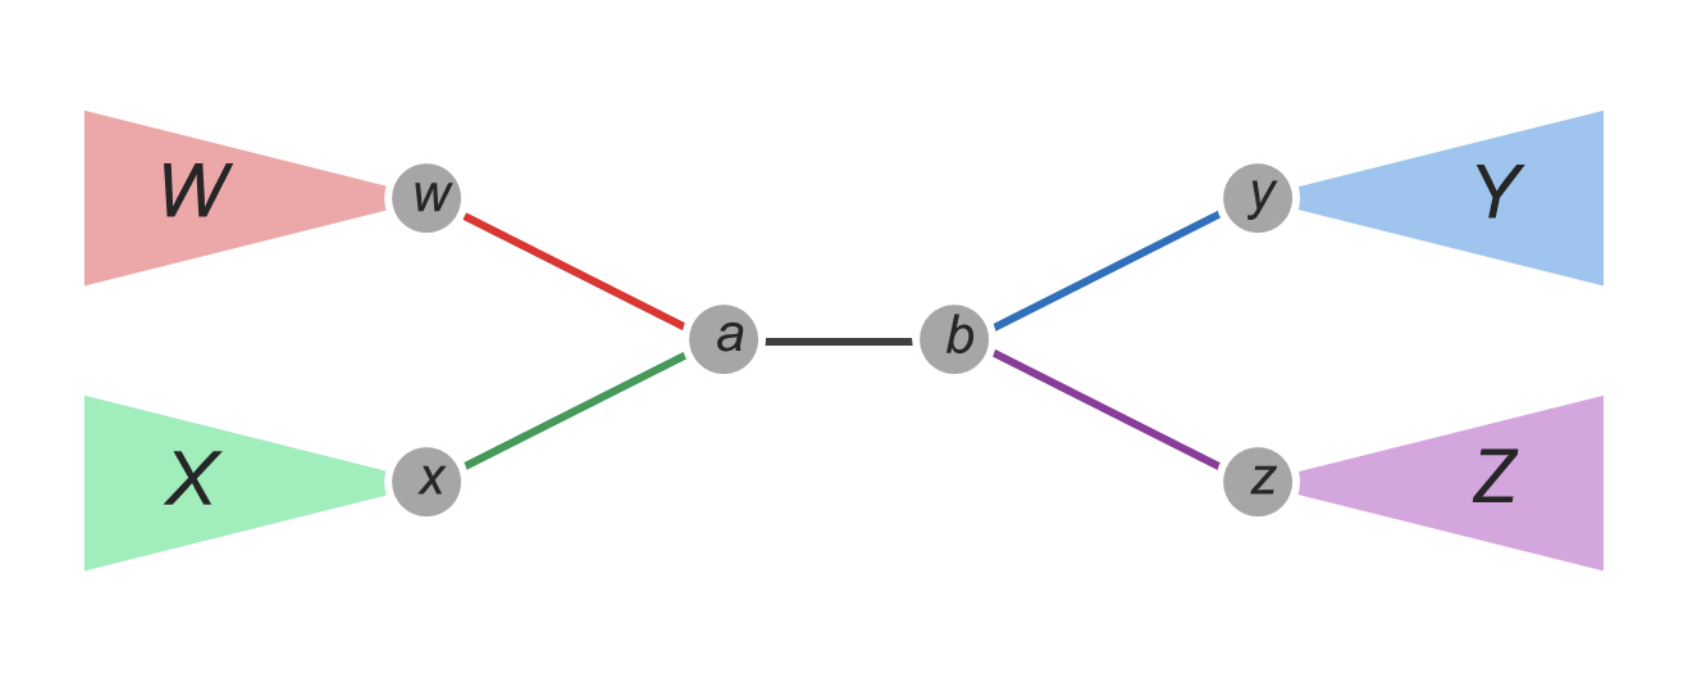
\includegraphics[width=0.7\textwidth]{poglavlja/7/slike/slika8.png}
\end{center}
\caption{Prikaz stvaranja \v{c}etiri podstabla}
\label{fig:pscp}
\end{figure}

Preure\dj enje rasporeda ovih stabala se naziva razmena najbli\v{z}ih suseda \ref{fig:psns}.

\begin{figure}[h!]
\begin{center}
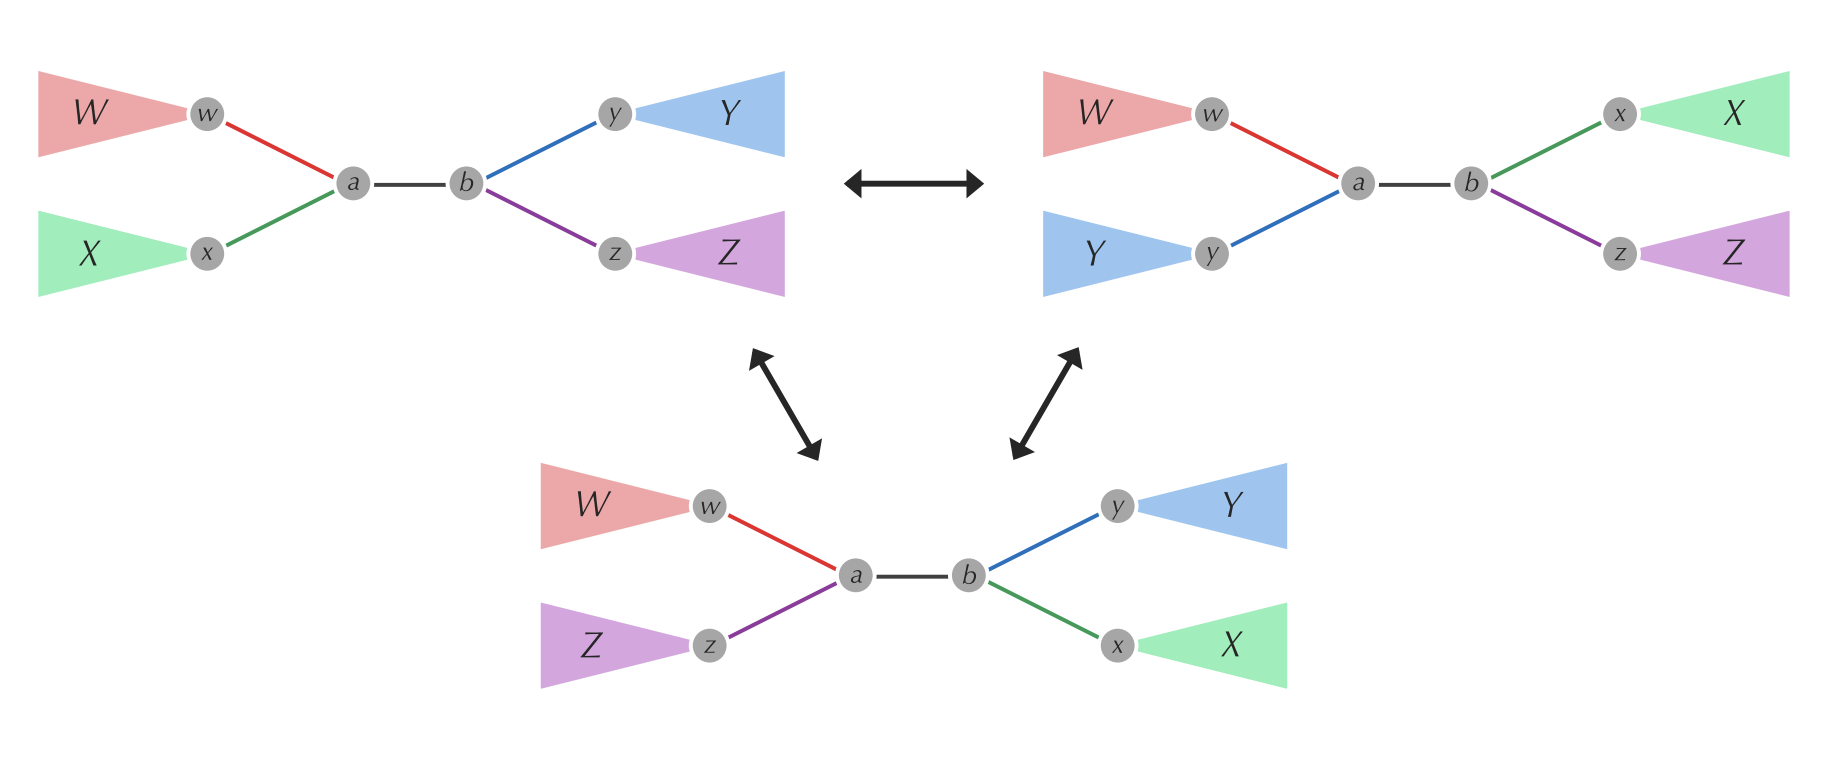
\includegraphics[width=0.7\textwidth]{poglavlja/7/slike/slika9.png}
\end{center}
\caption{Prikaz razmene najbli\v{z}ih suseda}
\label{fig:psns}
\end{figure}

\begin{tcolorbox}
\textbf{Problem najbli\v{z}ih suseda u stablu:} Za datu granu u binarnom stablu, generisati dva suseda ovog stabla. \\
Ulaz: Unutra\v{s}nja grana binarnog stabla.\\
Izlaz: Dva najbli\v{z}a suseda ovog stabla za datu unutra\v{s}nju granu.
\end{tcolorbox}


Heuristika za razmenu najbli\v{z}ih suseda:
\begin{enumerate}
	\item Postaviti trenutno stablo na koreno binarno stablo proizvoljne strukture.
	\item Pro\'ci kroz sve unutra\v{s}nje grane (a ne jednu kao malo pre) i izvr\v{s}iti sve mogu\'ce razmene najbli\v{z}ih suseda.
	\item Re\v{s}iti problem male parsimonije za svako takvo stablo.
	\item Ako stablo ima skor parsimonije bolje od optimalnog stabla, postaviti da to bude trenutno stablo; ina\v{c}e, vratiti trenutno stablo.
\end{enumerate}


\iffalse 
\newpage

\section{Zadaci sa vežbi}
\setexamplecodestyle

U nastavku će biti predstavljeni zadaci sa vežbi na kursu rađeni u programskom jeziku Python.

\subsection{Additive Phylogeny}

\lstinputlisting[language=Python]{poglavlja/7/kodovi/AdditivePhylogeny.py}

\subsection{UPGMA}

\lstinputlisting[language=Python]{poglavlja/7/kodovi/UPGMA.py}


\fi 